\section{Introduction}

For large-scale online service providers, such as Google, Facebook, and
Baidu, an important data communication pattern is {\em inter-DC
multicast} of bulk data--replicating massive amounts of data (e.g.,
user logs, web search indexes, photo sharing, blog posts)
from one DC to multiple DCs in geo-distributed locations.
%A common inter-DC communication pattern {\em bulk-data inter-DC multicast},
%which replicates data (e.g., user
%logs, search engine indexes, offline file sharing, forum posts, and
%databases) from one DC to any set of destination DCs.
Our study on the workload of \company shows that inter-DC multicast
already amounts to 91\% of inter-DC traffic (\Section\ref{sec:motivation}),
which corroborates the traffic pattern of other large-scale online
service providers~\cite{kumar2015bwe,zhang2016piebridge}.
As more DCs are deployed globally and bulk data are exploding,
inter-DC traffic then needs to be replicated in a frequent and efficient manner.
%Such latency requires to be short especially when hot issues occurs. Therefore, some services need to replicate large amount of data in a quite frequent and efficient way.
%, a key driving force
%behind recent efforts to improve inter-DC network performance
%(e.g.,~\cite{savage1999Theend,jain2013b4,kumar2015bwe,hong2013achieving,zhang2015guarantee}).


%Global-scale online services, such as Google, Facebook, and Baidu,
%depend crucially on the ability to distribute data across
%geo-distributed datacenters (DCs) in a timely and cost-effective
%manner. This has introduced substantial challenges, as data sizes
%continue to explode and more DCs are deployed to reach a global
%footprint.
%These trends have been a key driving force behind recent efforts
%to optimize the WAN performance between two
%DCs~\cite{b4,bwe,swan,??,??,??}.


\begin{figure}[t!]
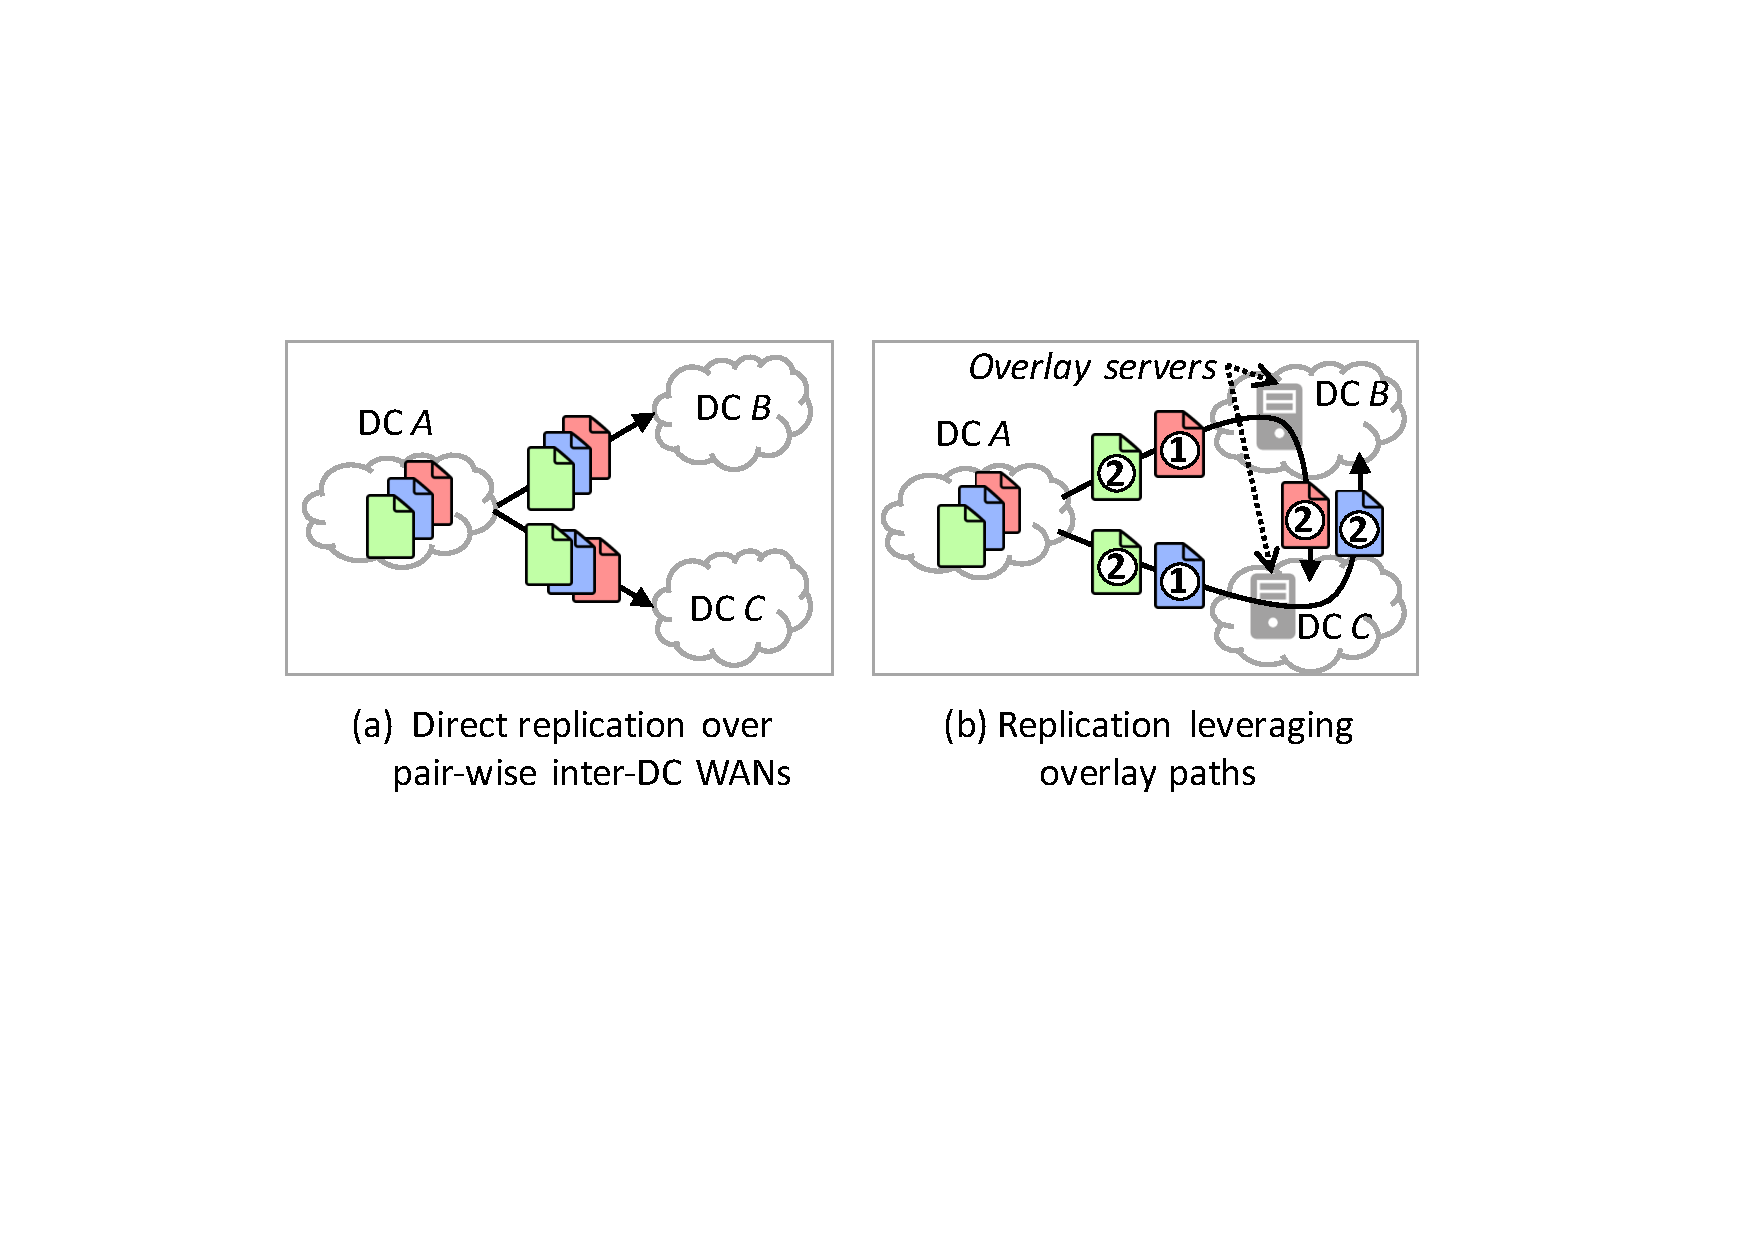
\includegraphics[width=83mm]{images/intro-example-3.pdf}
\vspace{-0.4cm}
\tightcaption{A simple network topology illustrating how
overlay paths reduce inter-DC multicast completion time.
%Assume the bottleneck is the outgoing router of DC $A$.
Assume that the WAN link between any two DCs is 1GB/s, and
that $A$ wants to send 3GB data to $B$ and $C$.
Sending data from $A$ to $B$ and $C$ separately
takes 3 seconds (a),
but using overlay paths $A$$\rightarrow$$B$$\rightarrow$$C$
and $A\rightarrow$$C$$\rightarrow$$B$
simultaneously takes only 2 seconds (b).
The circled numbers show the order for each data piece
 is sent. }
\label{fig:intro}
\vspace{-0.4cm}
\end{figure}

While there have been tremendous efforts towards better inter-DC
network performance (e.g.,~\cite{savage1999Theend,jain2013b4,
kumar2015bwe,hong2013achieving,zhang2015guarantee}), the focus has
been improving the performance of the wide area network (WAN) path
between each pair of DCs. These WAN-centric approaches, however, are
incomplete, as they fail to leverage the rich application-level
overlay paths across geo-distributed DCs, as well as the capability
of servers to store-and-forward data.
As illustrated in Figure~\ref{fig:intro}, the performance of inter-DC
multicast could be substantially improved by sending data in parallel
via multiple overlay servers acting as intermediate points to
circumvent slow WAN paths and performance bottlenecks in DC networks.
%(More examples can be found in \Section\ref{sec:motivation}.)
It is important to notice that these overlay paths should be {\em
bottleneck-disjoint}; that is, they do not share common bottleneck
links (e.g., $A$$\rightarrow$$B$$\rightarrow$$C$ and
$A$$\rightarrow$$C$$\rightarrow$$B$ in Figure~\ref{fig:intro}).
and that such bottleneck-disjoint overlay paths are available in
abundance in geo-distributed DCs.




This paper presents {\em \name}, an {\em application-level multicast
overlay network}, which splits data into fine-grained units, and
sends them in parallel via bottleneck-disjoint overlay paths. These
paths are selected dynamically in response to changes in network
conditions and the data delivery status of each server. Note that
\name selects application-level overlay paths, and is therefore
complementary to network-layer optimization of WAN performance.
While application-level multicast overlays have been applied in other
contexts (e.g.,~\cite{Liebeherr2002Application,Wang2007mTreebone,
Andreev2013Designing,Mokhtarian2015Minimum}), building one for
inter-DC multicast traffic poses two challenges. First, as each DC
has tens of thousands of servers, the resulting large number of
possible overlay paths makes it unwieldy to update overlay routing
decisions at scale in real time. Prior work either relies on local
reactive decisions by individual servers~\cite{kostic2003bullet,
Repantis2010Scaling,Huang2014A}, which leads to suboptimal decisions
for lack of global information, or restricts itself to strictly
structured (e.g., layered) topologies~\cite{Nygren2010The}, which
fails to leverage all possible overlay paths. Second, even a small
increase in the delay of latency-sensitive traffic can cause
significant revenue loss, so the bandwidth usage of inter-DC
bulk-data multicasts must be tightly controlled to avoid negative
impact on other latency-sensitive traffic.
%\myfootnote{Despite
%priority-based queuing at the ingress/egress points of each DC, the
%inter-DC traffic can still negatively impact latency-sensitive
%traffic performance, as they share the WAN links not managed by
%\company. This problem is so profound that some CDNs have built
%dedicated infrastructure as their inter-DC WANs, but in many cases,
%such as in \company's, DCs are connected through public ISPs}.

To address these challenges, \name fully {\em centralizes} the
scheduling and routing of inter-DC multicast. Contrary to the
intuition that servers must retain certain local decision-making to
achieve desirable scalability and responsiveness to network dynamics,
\name's centralized design is built on two empirical observations
(\Section\ref{sec:overview}):
(1) While it is hard to make centralized decisions in real time, most
multicast data transfers last for at least tens of seconds, and thus
can tolerate slightly delayed decisions in exchange for near-optimal
routing and scheduling based on a global view.
(2) Centrally coordinated sending rate allocation is amenable to
minimizing the interference between inter-DC multicast traffic and
latency-sensitive traffic.

The key to making \name practical is how to update the overlay
network in near real-time (within a few seconds) in response to
performance churns and dynamic arrivals of requests. \name achieves
this by {\em decoupling} its centralized control into two
optimization problems, scheduling of data transfers, and overlay
routing of individual data transfers. Such decoupling attains
provable optimality, and at the same time, allows \name to update
overlay network routing and scheduling in a fraction of second; this is four
orders of magnitude faster than solving routing and scheduling jointly
when considering the workload of a large online service provider (e.g., sending
$10^5$s of data blocks simultaneously along $10^4$ disjoint
overlay paths).


We have implemented a prototype of \name and integrated it in
\company. We deployed
\name in 10 DCs and ran a pilot study on 500~TB of data transfer
for 7 days (about 71~TB per day).
Our real-world experiments show that \name achieves 3-5$\times$
speedup over \company's existing solution named \alg, and it can eliminate the
incidents of excessive bandwidth consumption by bulk-data transfers.
Using trace-driven simulation and micro-benchmarking, we also show
that: \name outperforms techniques widely used in CDNs, that \name
can handle the workload of \company's inter-DC multicast traffic with
one general-purpose server, and that \name can handle various
failure scenarios.


Our contributions are summarized as followed:
\begin{packeditemize}
\item Characterizing \company's workload of inter-DC bulk-data
multicast to motivate the need of application-level multicast
overlay networks (\Section\ref{sec:motivation}).
\item Presenting \name, an application-level multicast overlay
network that achieves near-optimal flow completion time by a
centralized control architecture
(\Section\ref{sec:overview},\ref{sec:logic},\ref{sec:system}).
\item Demonstrating the practical benefits of \name by a real-world
pilot deployment in \company (\Section\ref{sec:evaluation}).
\end{packeditemize}
